\chapter{介绍}{1}


        发明家们一直梦想着做出能思考的机器。这种愿望可以追溯回古希腊时期。皮格马利翁\footnote{善雕刻的国王},代达罗斯\footnote{希腊名建筑师},赫菲斯托斯\footnote{火神}等神话形象可以被认为是传奇的发明家;而嘉拉迪雅\footnote{皮格马利翁的雕刻作品,化身为人},塔洛斯\footnote{代达罗斯外甥,向他学艺成为大师},潘多拉\footnote{赫菲斯托斯用泥土造的女人}则可以被认为是人造生命。


当人们第一次设想制造可编程计算机时,就在想能否使它们变得智能,而可编程计算机在100多年之后才问世\footnote{Lovelace,1842,被视为第一位给计算机写程序的人}。今天,人工智能(AI)是一个有许多实际应用和活跃研究课题的热门领域。而且我们希望智能软件可以自动完成日常劳动,理解语音和图像,进行医学诊断和支持基础科学研究。


在人工智能发展的早期,AI迅速的解决了那些对人类来说困难但对计算机而言相对简单的问题,这些问题可以明确的被一系列的公式和数学规则所定义。而人工智能面临的真正挑战后来变成了解决对人类来说执行起来容易但定义规则困难的问题。这些问题就像理解语言,或识别人脸,对人类而言感觉像自动的,仅凭直觉就能处理的。

本书探讨的是解决上述问题的方法。这类方法允许计算机通过建立层级概念从经验中学习和理解世界,而每个概念由一系列与其相关且更简单的概念组成。通过从经验中获取知识,这类方法避免了人工的指定计算机所需要的知识。概念的层级性使得计算机可以通过简单的概念学习更为复杂的概念。如果我们画出概念是如何组织和建立的,这幅画会有很多层级,会很深。因此,我们将这类方法称为深度学习。


许多早期的成功的AI大多是应用在相对简单和有规律的环境中,并不要求计算机对环境有过多认知。 例如,IBM的深蓝系统在1997年打败过国际象棋的世界冠军Garry Kasparov。国际象棋是一个非常简单的世界,因为他的32个棋子必须在64个棋格中严格按照规律移动。找到一个成功的下棋策略当然是一个非常大的成功,但其挑战并不在于描述下棋的位置和移动的方向。国际象棋可以被一系列简单有条理的规则提前被程序员定义。


有些嘲讽的是,那些对于人类很难解决的规则化和抽象的任务对于计算机来说恰恰是比较容易的。计算机很久之前就已经打败了国际象棋的人类冠军,但仅仅到近年才能在识别图像和语音上能稍微和人类的平均水平匹敌。人的日常生活需要对真实世界的大量认知。许多知识对我们而言是主观的和本能的,因此很难通过正式的方式明确的表达出来,而计算机需要这类知识来使其表现的更加智能。AI的关键挑战之一就是如何使计算机学习到这些非结构化的认知。

一些AI的项目曾经试图将知识以硬编码的方式写入专门的语言中,计算机使用逻辑和规则推理这些语言中的语句,这种方法被称为“知识库”。然而,这些项目都没有获得巨大的成功。其中最著名的是Cyc, Cys是一个推理引擎,CycL是其专有的知识语言库,人通过繁重的工作将知识语言录入CycL中。他们企图通过足够复杂的规则来精确的描述这个世界,但结果不尽如人意。比如,Cyc不能正确的理解Fred在早上刮胡子这个故事。推理引擎捕捉到了故事中的矛盾:它知道人类并没有电动的组成部分;但由于Fred拿着电动剃须刀,使得推理引擎认为Fred是一个包含电动部分的实体。因此,推理引擎不知道此时Fred是否还是人类。

上述的硬编码的知识系统的失败表明,AI需要从原始的数据中提取模式并学习知识,这种能力被称为“机器学习”。机器学习的引入使得计算机能够处理真实世界的问题并作出主观性的决策。一种叫做“logistic回顾”的简单机器学习算法可以决定是否推荐剖腹产,一种“叫做朴素贝叶斯”的简单机器学习算法可以做垃圾邮件的分类。


上述的简单机器学习算法非常的依赖输入数据的表现形式。比如,当logistic 回归被用于是否推荐剖腹产的时候,这个算法并不直接检查孕妇,而是通过医生输入的血压、病史等相关参数来做决策。每个参数被称为一个特征。logistic 回归知道每个特征和最后输出的关联,然而,他不能影响特征被定义的方式。 如果给出一个孕妇的核磁共振结果而非是医生的结构化的参数报告,logistic 回归就不能得出有意义的结果了。核磁共振扫描结果上的每个独立像素和生产中的可能发生的并发症的相关性十分微小。


对特征表达形式的依赖是计算机科学甚至日常生活中的一个普遍现象。 在计算机科学中,如果数据按照某种格式组织索引,搜索工作会获得指数倍的效率提升。人们能够很容易的对阿拉伯数字做运算,而对罗马数字的运算会耗费更多时间。所以特征的表达对于机器学习算法可能产生的巨大影响也不足为奇了。图\ref{fig:represent}展示了一个直观的例子。
\begin{figure}[htbp] %  figure placement: here, top, bottom, or page
   \centering
   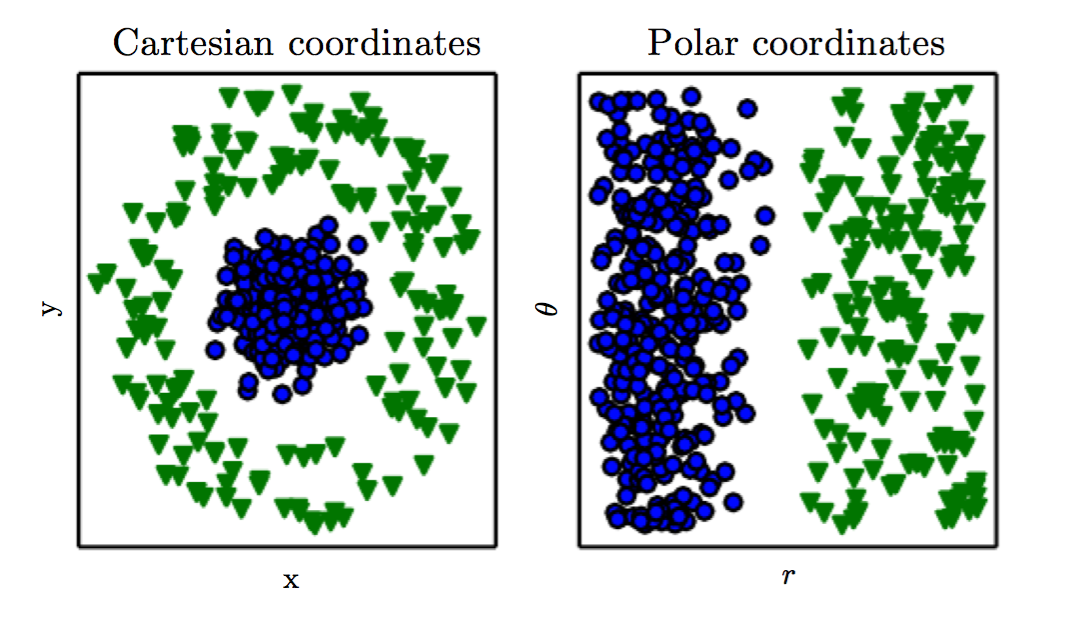
\includegraphics[width=4in]{fig/chap1/represent.png} 
   \caption{不同的表达形式的例子:假设我们要在如上散点图中画一条线分割两个不同种类的数据,左图是笛卡尔坐标系中的散点图,这个任务是不可能完成的。右图是该数据在极坐标系中的散点表示,这个任务可以通过画一条垂线就完成了。}
   \label{fig:represent}
\end{figure}

许多人工智能的任务可以通过手工设计合适的特征组并输入一个简单的机器学习模型来完成。比如,说话人的声道大小是说话人识别任务的一个有用的特征,他可以作为说话人是男人、女人或是小孩的一个强线索。


然而,对许多任务来说,我们很难去发现应该抽取什么样子的特征。比如,我们需要在一张照片中检测车辆。我们知道汽车有轮子,所以我们可能会把轮子作为汽车检测的一个特征。不幸的是,在像素的级别上描述轮子是非常困难的。轮子的几何形状非常简单,但是轮子上的阴影、金属部分的折射、保险杠的影响或前景物体的遮挡等让描述它变得非常复杂。


上述问题的一个解决方案是,我们不仅使用机器学习的算法去学习特征表达到输出结果之间的映射,也使用机器学习去学习起特征表达,这种方案被称为“表征学习”。表征学习通常可以获得比手工特征更好的表现,它也让AI系统在很少的人工干预下可以快速的适应新的任务。表征学习算法可以为一个简单的任务在数分钟之内找到一组好的特征,复杂的任务耗时则从几小时到几个月不等。为一个复杂的任务人工的设计特征需要耗费大量的时间和精力,甚至可能花费整个研究团队数十年的时间。


表征学习的一个经典算法叫做“自编码器”。自编码器有两部分组成:编码器把输入的数据转换到不同的表征空间;解码器把这个表征再转换回原始的数据。自编码器的训练目标一个是在不断的编码和解码的过程中保存尽量多的信息,另一个是在表征空间中有良好的属性。不同的任务需要自编码器有不同的属性。


不管是手工特征还是学习的特征,我们的目标通常是分离出观测数据的“变化因子”。在本文中,我们使用“因子”来表示不同的影响源,这些因子通常都不是通过乘法来组合的,这些因子也通常不能通过直接观测来量化。相反的,这些因子或许存在在物理世界中尚未发现的物体或力量中但对可观测的量造成了影响。这些因子也可能存在于人类大脑的结构中,提供对可观测数据的推理和抽象解释能力。当分析一段录音时,变化因子包括说话人的年龄、性别、口音和他所说的一字一句。当分析一幅汽车的图像时,变化因子包括车的位置、颜色、阳光的角度和亮度。


许多真实世界的AI应用面对的主要问题来源就是许多的变化因子影响着我们观测到的每一份数据。图像上一辆红色的车的像素值在夜晚的时候会非常靠近黑色。汽车的轮廓表现在不同的观测角度下是不同的。绝大多数的应用都需要我们对变化因子解耦并且丢弃那些我们不关心的变化因子。


从原始数据中抽取如上所说的高层次和抽象的特征固然是非常难的。如说话人口音在内的许多变化因子,都需要对数据具有非常精致和复杂、接近人类的理解能力才能获取。当获取一个合适的特征表达的难度几乎和解决原始问题相当的时候,表征学习似乎并不能给我们带来帮助。


“深度学习”通过表征的层级组合解决了表征学习中的核心问题。深度学习允许计算机通过学习一系列简单的概念来组成复杂的概念。图\ref{fig:deep_learning_intro} 展示了深度学习如何从图像中通过一些如边缘,角点,轮廓的简单的特征组合来表示一个人的。

\begin{figure}[htbp] %  figure placement: here, top, bottom, or page
   \centering
   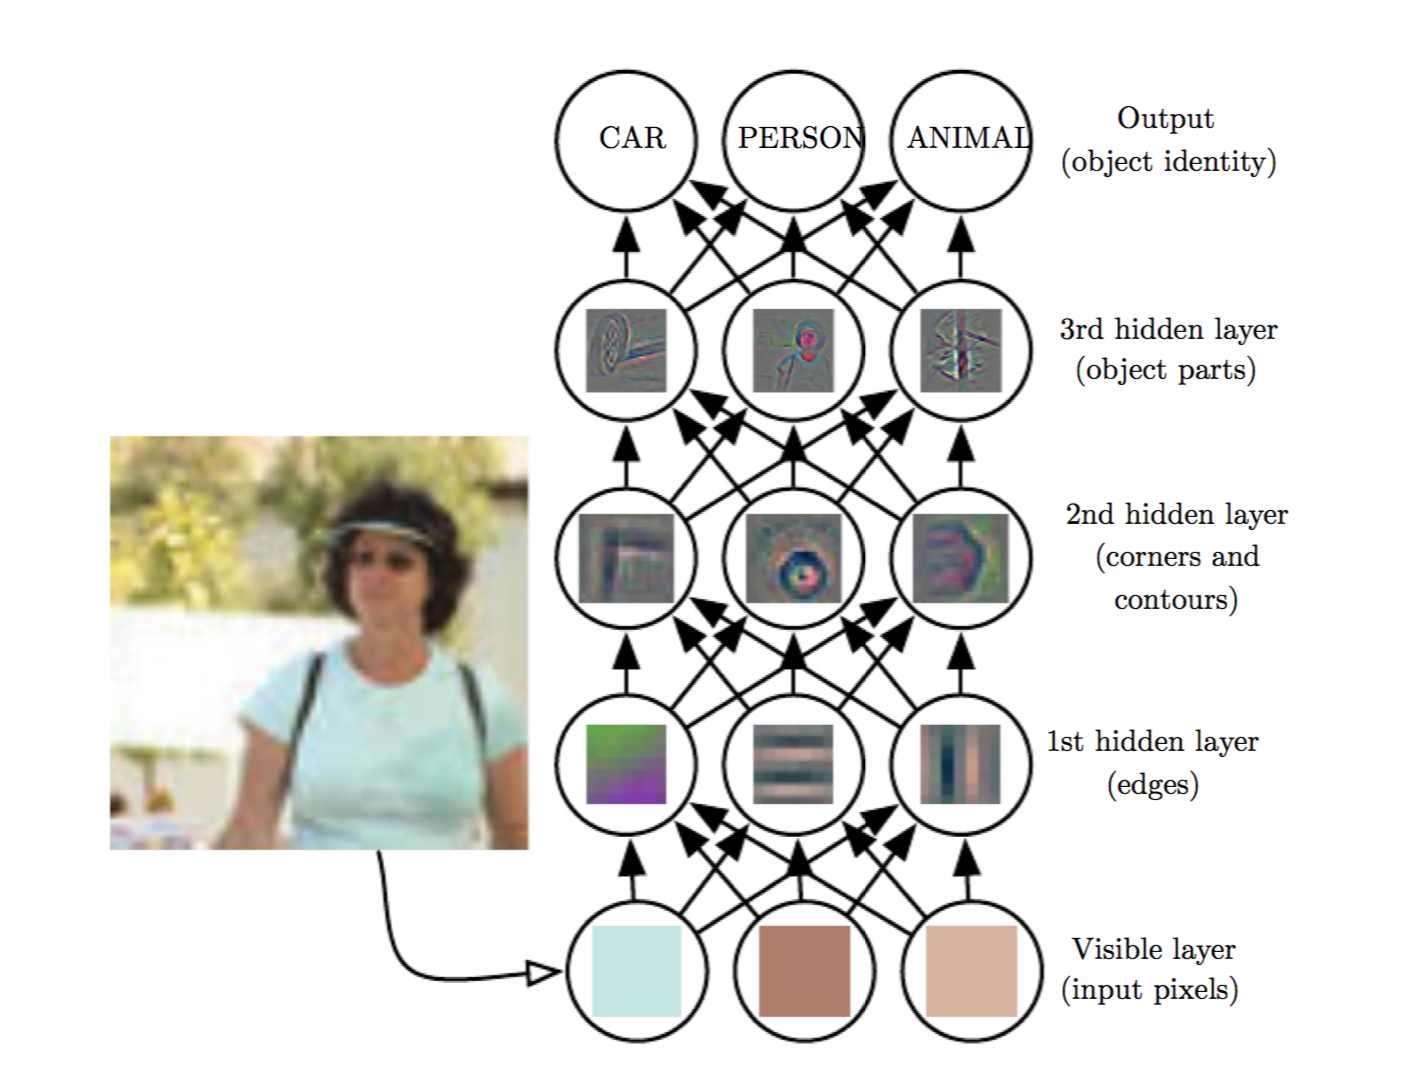
\includegraphics[width=5in]{fig/chap1/deep_learning_intro.png} 
   \caption{深度学习模型图解。对计算机而言,理解如像素值等的传感器捕获的原始数据是非常困难的。从一组像素值到物体标签的函数映射是十分复杂的,如果直接来学习或评估这个映射看起来是个不可能的。深度学习通过把这个复杂的映射分解成一系列的简单映射来解决这个问题,每个简单的映射是模型中一个不同的“层”(layer)。原始的数据输入被称为“可视层”,因为它包含着我们观察地到的变量。紧接着是一系列的“隐层”不断的从图像中抽取抽象的特征,这些层被称为“隐层”是因为他们的值不是由原始数据直接给出的,模型需要决定哪些概念对解释可观测数据之间的关联是有用的。图示为每个隐层所学习到的概念的可视化。第一个隐层可以十分容易的通过相邻像素之间的明暗对比抽取出边缘的信息,第二层则可以通过轮廓信息学习出角点和轮廓的信息,第三层则可以通过角点和轮廓的信息寻找到指定物体的一些部件信息。最终,通过对物体的部件描述,我们可以识别出图像中的物体。}
   \label{fig:deep_learning_intro}
\end{figure}


前馈神经网络或多层感知机(MLP)是深度学习的一个典型例子。多层感知机不过是把输入映射到输出的数学函数,而这个函数是由许多更简单的函数组成的,且我们可以认为应用不同的数学函数可以提供对输入数据的不同表征。


学习合适的表征是深度学习的一方面,另一方面是“深度”允许计算机学习到分步的计算过程。每一层的表征都可以被认为是计算机并行的执行了一系列的指令集后的记忆状态,更深层次的网络可以按照序列顺序执行更多的指令集。序列的指令拥有更强大的能力,因为它可以从前序的指令的结果中获得参考。根据深度学习的这些观点,并不是层中激活的所有信息都可以编码对解释输入数据的起作用的变化因子。表征会存储有利于算法执行、使得输入有意义的状态信息。在传统计算机程序中,状态信息可以类比于计数器或者指针,它与输入内容没有直接的关系,但是可以帮助深度学习模型组织其自身的处理过程。


有两种主要的方法可以测量一个模型的深度。第一种是统计在测试网络的过程中必须被执行的序列指令的数量,可以认为这是描述模型从输入到输出的流程图中的最长路径。就像相同的程序由于编程语言的不同会有不同的长度,对于同一个函数,其在流程图中的长度取决于我们把哪些步骤看作是独立的。图\ref{fig:flow_chart}描述了不同的语言是如何使得同一个结构拥有不同的深度。

\begin{figure}[htbp] %  figure placement: here, top, bottom, or page
   \centering
   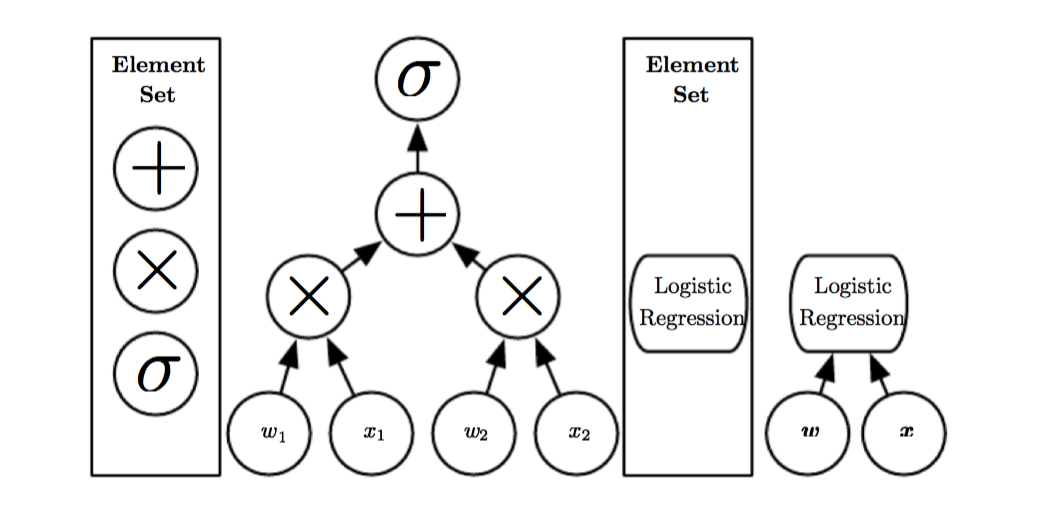
\includegraphics[width=5in]{fig/chap1/flow_chart.png} 
   \caption{每一个节点表示一个不同的操作,图示为从输入到输出映射的计算图。深度是从输入到输出的最长路径,但它的计算依赖于对独立计算步骤的定义。上图描述的是逻辑回归的模型$\delta(w^Tx)$,$\delta$是逻辑回归的sigmoid函数。如果我们认为加法、乘法和sigmoid操作是计算机语言的元素级操作,那这个模型的深度就是3;如果我们认为逻辑回归本身就是就是元素级操作,那这个模型的深度就是1。}
   \label{fig:flow_chart}
\end{figure}


另一个由深度概率模型所使用的概念是,深度并不是计算流程图的深度,而是描述概念之间的层级结构的组织图的深度。在这个概念中,由计算流程图得到的深度往往比概念组织图得到的深度要深得多。比如,一个AI系统如果在观测一副有一只眼睛在阴影中的人脸图像时可能刚开始只能观测到一只眼睛,等到能发现整个人脸的时候,AI可能会推理出另一只眼睛也是存在的。在这个例子中,概念组织图只有两层:一层是检测眼睛,一层是认知人脸;但如果我们n次调优每一层概念时,计算流程图中则有2n层。


该选择计算流程图还是概念组织图来计算深度是没有定论,而且每个人选择构建图所使用的最小元素也不尽相同,因此对一个架构来说并没有一个唯一的正确深度,就像对计算机程序来说也没有一个唯一的正确深度。同样,对于一个模型来说,多深才叫“深”也没有定论。可以肯定的是,相比传统的机器学习来说,深度学习可被认为是一种含有大量计算的函数学习和概念学习的模型。

总之,本书的主题“深度学习”是AI的一种实现方法,而且它也是一种可以使得机器自身通过数据和经验不断提升的机器学习方法。本书的作者们认为,深度学习是构建在真实世界处理复杂问题的AI系统的目前唯一可行的方法。深度学习是机器学习中很强大很灵活的一种方法,因为它学习的是如何将真实环境中的任务以嵌套的层级概念表达出来,通过这些嵌套的概念,它可以将底层的表征不断抽象为含有语义的更高层的特征。图\ref{fig:ai_approach}显示了不同的AI方法之间的关联,图\ref{fig:ai_discipline}概括了这些方法是如何实现的。

\begin{figure}[htbp] %  figure placement: here, top, bottom, or page
   \centering
   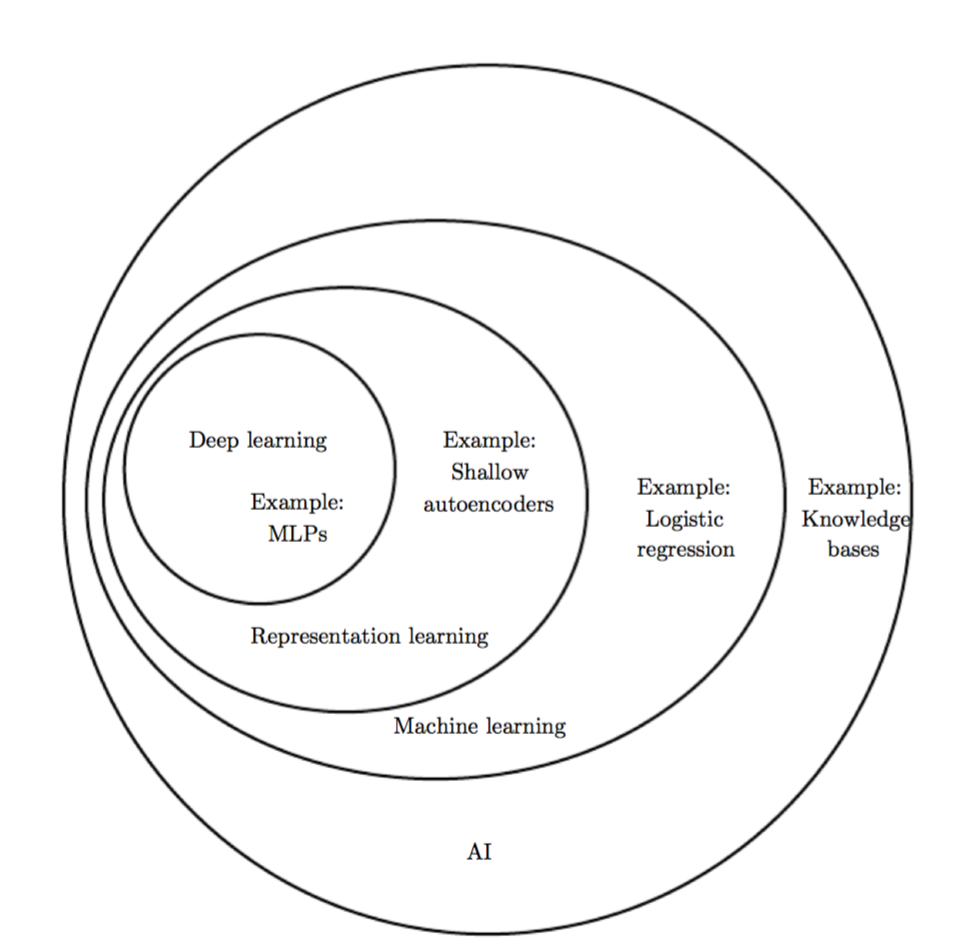
\includegraphics[width=6in]{fig/chap1/ai_approach.png} 
   \caption{这个维恩图解释了为什么深度学习也是一种表征学习的方法和机器学习方法。维恩图的每个部分都给出了一个AI方法的实例。}
   \label{fig:ai_approach}
\end{figure}

\begin{figure}[htbp] %  figure placement: here, top, bottom, or page
   \centering
   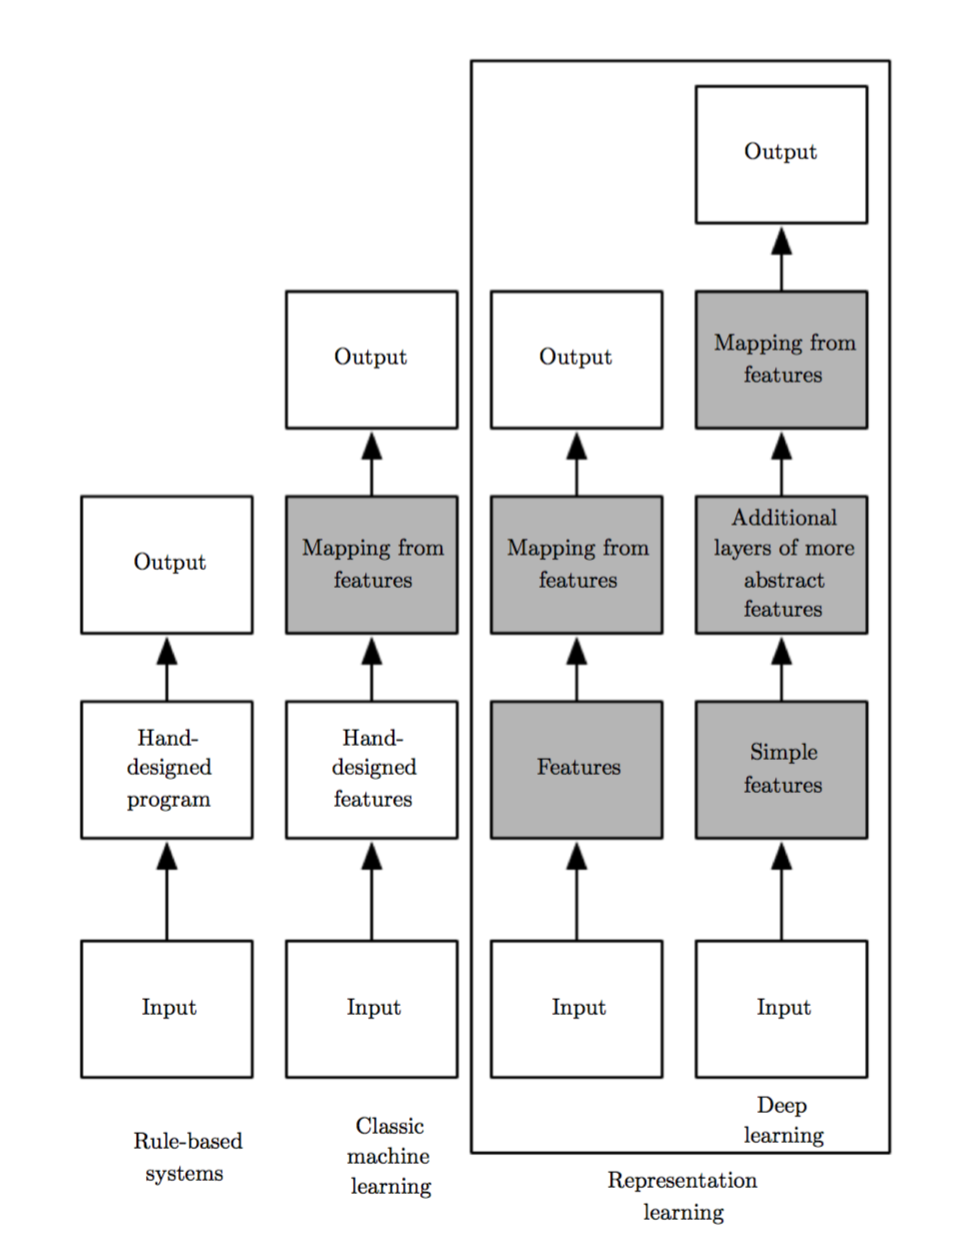
\includegraphics[width=4in]{fig/chap1/ai_discipline.png} 
   \caption{此图显示了不同的AI算法是如何组成AI系统的不同部分的。深色的框表示这个模块是可以从数据中学习的。}
   \label{fig:ai_discipline}
\end{figure}

\section{谁应该读这本书}

这本书对很多类型的读者都有用处,但我们主要为两类读者而写。一类是正在学习机器学习的本科生或研究生,或准备开始在深度学习和人工智能的研究领域大展身手的人。另一种是想要快速把深度学习技术应用在他们的产品中,但没有机器学习或统计背景的工程师。深度学习已经在多个软件领域中获得了成功,包括计算机视觉、语音识别、自然语言处理、机器人、生物信息学和化学、视频游戏、搜索引擎、在线广告及金融等。


为适应尽可能多的读者,本书主要由三部分构成。第\ref{part:1}部分介绍基础的数学工具和机器学习的概念。第\ref{part:2}部分介绍了最为广泛使用的深度学习算法。第\ref{part:3}部分介绍了被认为对深度学习的进一步研究十分重要的更又去的想法。


读者可以根据自身的背景或感兴趣的方向自由的阅读本书。对线性代数、概率和基础机器学习算法熟悉的读者可以跳过第\ref{part:1}部分,而只想实现一个可用的深度学习系统的读第\ref{part:2}部分就够了。图\ref{fig:1.6}提供了本书的一个高层的组织流程图。


我们写本书的时候假设本书的读者都具有计算机科学的相关背景,因此我们也认为大家都熟悉编程、对计算性能和算法复杂度有基本认识、有入门级的微积分和图论的知识。

\begin{figure}[htbp] %  figure placement: here, top, bottom, or page
   \centering
   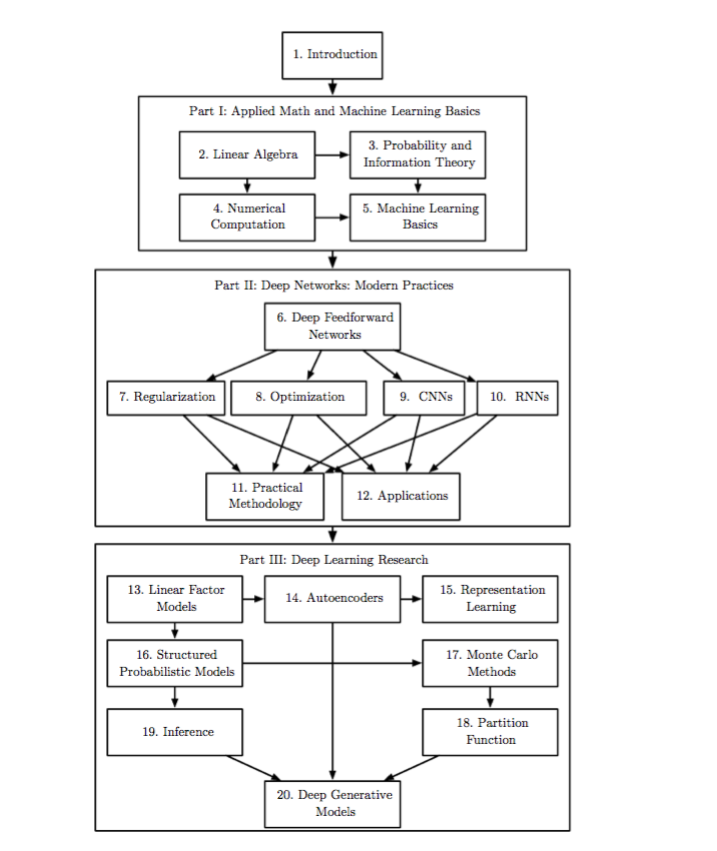
\includegraphics[width=7in]{fig/chap1/1.6.png} 
   \caption{本书的组织图。如果箭头从第A章指向第B章,意味着理解章节B的需要A的知识。}
   \label{fig:1.6}
\end{figure}


\section{深度学习历史趋势}
伴随着历史的轨迹来看深度学习是最荣易让人理解的一种方式。我们找出了一些深度学习发展的关键趋势而非提供一个详尽的发展历史:

\begin{itemize}
\item 深度学习有着悠长和丰富的历史,也有许多人抱持着不同的哲学观点,但它的发展并非一帆风顺。
\item 当可以获取的训练数据逐步增长时,深度学习的成效也在增长。
\item 当适用于深度学习的软硬件提升时,深度学习模型的大小也在增长。
\item 深度学习解决复杂问题能力和精确度随着时间不断提升。
\end{itemize}

\subsection{改变神经网络命运的人们}
我们期待着本书的读者听说过深度学习这个令人兴奋的新技术,能非常惊喜的看到有一本书在介绍这个新兴领域的历史。事实上,深度学习在1940年左右就已经出现。深度学习显得很新是过了很多年前它并不十分流行,而且它有许多不同的名字,直到最近才被称为深度学习。深度学习被多次更名,这也可以反映出不同的研究人员和不同的角度观点带来的影响。


本书并不意在介绍深度学习的全面历史,但是一些基础的认知可以帮助我们理解深度学习。广泛的说,深度学习的发展有三次浪潮:深度学习在1940-1960年间被认为是“控制论”,在1980-1990年间被称为“联结学”,从2006年后才被称为深度学习。这在图\ref{fig:1.7}中量化的表示了。


一些早期的学习算法在今天我们认识到其实是生物学习的计算机模型,即模仿大脑学习的机制。因此,深度学习的一个别名就是人工神经网络(ANNs),与之一致的观点是深度学习模型是受生物大脑启发的一个工程系统(人类大脑或其他动物的大脑)。这种机器学习中使用的神经网络有时候也会被用来理解大脑运行的机制,但这些网络一般没有被设计成实现生物机理的真实模型。从神经角度看深度学习的观点主要有两个思想。一个是大脑证明了智能的行为是可能的,一个直观的想法就是发现大脑运行背后的计算规则并复制其能力。另一种观点是,理解大脑和人智力背后隐含的原理是非常令人感兴趣的,所以揭示了这些基础科学问题的机器学习模型除了解决工程应用的问题外也是非常有意义的。


现代所说的深度学习已经超越了神经角度描述的任何种类的机器学习模型,它成为了一种更为普世的学习多层结构的指导原则,可以被应用于非神经学启发的机器学习模型构建。

\begin{figure}[htbp] %  figure placement: here, top, bottom, or page
   \centering
   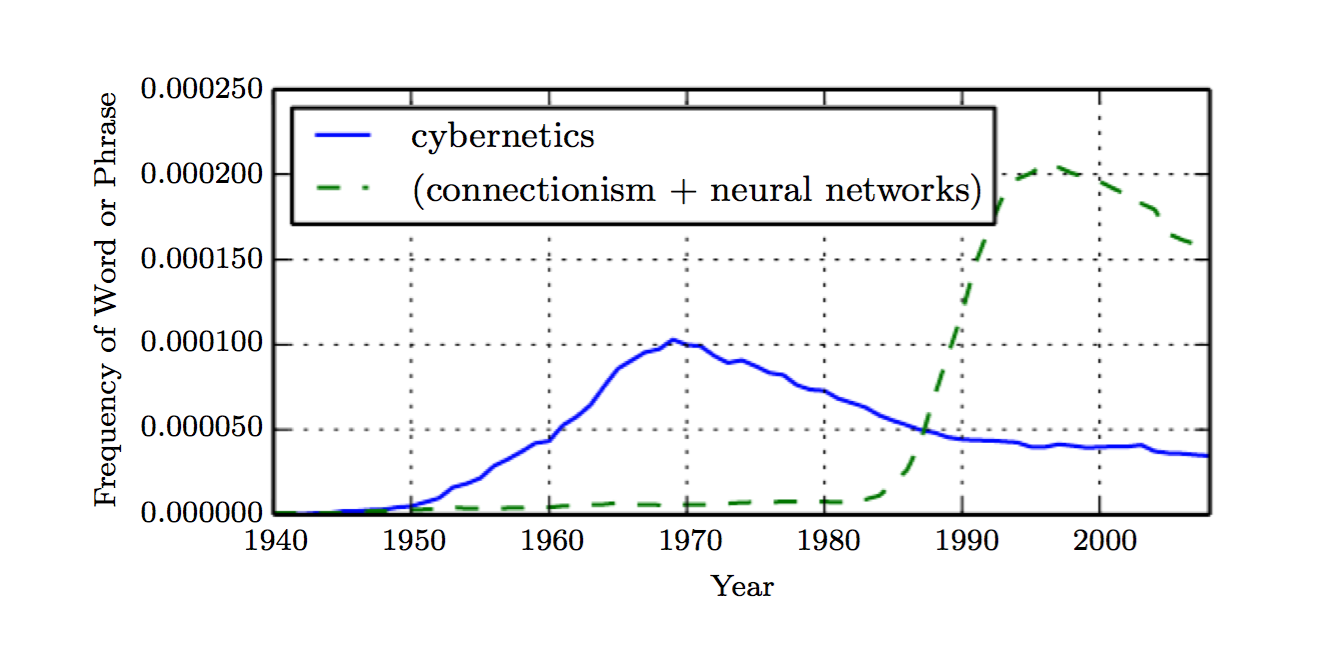
\includegraphics[width=4in]{fig/chap1/1.7.png} 
   \caption{本图展示了人工神经网络研究的发展史上三次浪潮中的两次,根据Google Books 中提到控制论、联结学或神经网络的批量得出的测量(第三次浪潮是最近才出现的)。第一次浪潮是在1940-1960间出现的控制论,伴随着生物学习理论的发展和第一个允许训练的单个神经元的感知元模型的建立。第二次浪潮是1980-1995年出现的联结学,那时出现了反向传播算法,我们可以训练拥有一到两个隐层的神经网络了。现在是第三次浪潮,从2006年开始的深度学习,直到2016年才被写进书中。不过另外两次浪潮也一样,也是滞后于相关科技的发展很长时间才被书中收录。}
   \label{fig:1.7}
\end{figure}


现代深度学习的先驱是受神经学启发的简单线性模型。这类模型有$n$个输入$x_1,...,x_n$和一个输出$y$,目标是学习一组权重$w_1,...,w_n$使得$f(\textbf{x},\textbf{w}) =x_1w_1+...+x_nw_n$。第一次神经网络研究的热潮如图\ref{fig:1.7}所示,被称为控制学。

McMculloch-Pitts神经元是一个描述大脑功能的早期模型,这个线性模型可以通过$f(\textbf{x},\textbf{w})$输出的正负来做二分类,当然,权值需要根据分类任务的不同进行相应的调整,而这些权值是需要人工设置的。直到1950年代,感知机出现了,它是第一个可以根据不同类别的数据对权值进行自动调整的模型。与此同时出现的自适应线性元件(ADALINE),通过简单地返回函数$f(\textbf{x})$来预测一个实数,也具有从数据中学习预测数字的能力。

这些简单的学习算法极大的影响了现代机器学习算法的版图。用于训练ADALINE的算法叫做随机梯度下降,经过稍微修改的随机梯度下降算法是目前绝对主流的深度学习训练算法。


感知机和ADALINE使用的$f(\textbf{x},\textbf{w})$类型的模型被称为线性模型。这类模型至今仍然被广泛的使用着,但如今的训练方法很多时候和最初的训练方法不同。


线性模型有许多局限性。最著名的一个是他不能学习异或函数,即$f([0,1],\textbf{w}) =1$ 且$f([1,0],\textbf{w}) =1$,但$f([0,0],\textbf{w}) =0$且$f([1,1],\textbf{w}) =0$。发现了线性模型这一缺陷的批评家引起了普遍性对生物启发学习的反弹,引起了第一次神经网络热度的退潮。


现在,神经科学仍然被认为是深度学习的一个重要灵感来源,但它已经不再被认为是这个领域的绝对指南。


今天,神经科学对深度学习研究的影响逐渐减弱,因为我们没有足够关于大脑运作机制的信息可以给出指导。如果要深刻理解大脑使用的算法,那就必须同时观测成千上万互相连接的神经元的活动,然而我们做不到这些。因此,我们和理解最简单和被研究的最透彻的大脑部分都相距甚远。


神经科学使得我们希望用一个深度学习的模型来解决不同的问题。神经学家发现雪貂可以利用大脑的声音处理区域学会“看”,如果这个区域被输入视觉信号的话。这证明了多数哺乳动物也许是使用某种单一的算法来使得大脑解决不同的问题。在这个假设出来之前,机器学习的领域是碎片化的,来自不同社区的研究人员在研究不同的领域,如自然语言处理、计算机视觉、运动规划和语音识别等。如今,这些社区仍然是独立的,但深度学习的研究团队可能会同时研究上面所说的许多领域。


我们可以从神经科学中得到一些粗略的指导。如通过不同计算单元的联结来使得系统变得智能就是受到大脑的启发。Neocognitron创造的一种处理图像的强大模型框架的灵感就来自于哺乳动物的视觉系统,随后这个模型成为了现代卷积网络的基础框架,这个模型在第章会再详细介绍。目前所使用的神经网络绝大多数建立在一个叫做\emph{线性整流单元}的模型基础上, Cognitron提供了一个更复杂的模型,这个模型也是受到大脑运作机制的启发而来。现代这个简化版本是由许多的观点整合而来的,如Nair、Hinton、Glorot就援引了神经科学的观点,Jarrett就更多的从工程角度进行了援引。神经科学虽然是一个重要的灵感源泉,但它不需要被视为刚性的指导。我们知道真实的神经元与线性整流单元的运算机制不尽相同,但更为写实的神经元工作机制并没有给机器学习带来很大的提升。虽然神经科学成功的激发了一些神经网络\textbf{结构}的建立,但我们现在对神经元的学习机制的掌握还不够,还不足以为训练这些结构的\textbf{学习算法}带来足够的指引。


媒体经常强调深度学习和大脑有多么相似。虽然深度学习的研究者和其他机器学习领域的研究者相比更容易引用脑科学的文章,但我们不应该把深度学习看做对大脑的一种模拟。现代深度学习从许多领域汲取养分,特别是一些应用数学的领域,如线性代数、概率论、信息论以及数值优化等。当一些深度学习研究人员援引神经科学作为一种重要灵感源泉时,另一些研究人员或许压根不关心神经科学。


理解大脑在算法级别的运作的工作是值得关注的。这类工作被称为是“计算神经科学”,是不同于深度学习的一个研究领域,许多研究者会在这两个领域之间游走。深度学习的领域主要关心的是如何建立具有可解决问题的智能系统,而计算神经科学的领域的重点工作是建立大脑运作的更精确的模型。


在1980年代,迎来了神经网络研究的第二次热潮,这次热潮主要是通过\emph{联结学}或\emph{并行分布式处理}的运动产生。联结学在认知科学中产生,认知科学是一种为了理解大脑的跨学科研究,并且有许多不同的层面的分析。在1980年代早期,许多认知科学家都在研究符号推理,尽管符号推理很流行,但是符号模型是如何用神经元在大脑中实现的都难以解释。联结学家就开始研究那些可以被神经元实现的认知模型,复兴了心理学家Donald Hebb在1940年代提出的许多想法。


联结学的核心思想就是通过联结许多简单的计算单元可以实现智能。这个洞见也适用于生物神经系统的神经元和计算模型的一些隐藏单元。


1980年代联结学运动中产生了一些核心观念对今天的深度学习来说仍然至关重要。


其中一条概念就是\emph{分布式表达}。这个概念描述的是每个对系统的输入都应该由许多的特征来表达,而每个特征都应该参与到许多的输入的表达。比如,我们有一个可以识别汽车、卡车、鸟的视觉系统,我们识别的物体可能是红的、绿的或者蓝色的。一种表达这些输入的方式是,我们有许多独立的神经元组或隐藏神经元组来处理九种不同的排列组合:红卡车、红汽车、红鸟、绿卡车、绿汽车等。这需要九个不同的神经元组,而且每一组都需要独立的学习相关的物体和颜色的概念。一个提升效能的方法就是使用分布是表达,使用三组神经元描述颜色,三组神经元描述物体信息,这样就只需要六组神经元而非九组。学习红色的神经元可以从汽车、卡车和鸟的图像中学习,而不限于特定的类型。分布式表达对本书非常重要,会在第\ref{chap:15}章进行更详细的描述。


另一个联结学运动的主要成就是成功的运用了反向传播来训练深度神经网络,并使得反向传播算法流行起来。这个算法在历史的流行度上有过跌宕起伏,但在目前深度学习的领域占了绝对的主导地位。

在1990年代,研究者们在使用神经网络进行序列模拟方面取得了很大的进步。Hochreitrt和Bengio解决了建模长序列的几个关键数学难题,在第\ref{sec:10.7}中会提到。Hochreiter和Schmidhuber提出了长短期记忆网络(LSTM网络)来解决序列建模中遇到的一些难题。如今,LSTM广泛的应用在很多序列建模的任务中,比如Google就使用它来做一些自然语言处理的工作。


神经网络的第二次浪潮一直持续到二十世纪九十年代中期。风险投资公司在寻求基于神经网络的和其他AI技术的投资机会时,往往会提出十分具有野心但不切合实际的要求。当AI的研究不能满足这些不合理的期望时,投资者会感到失望。而与此同时,机器学习的其他领域取得了进步。核方法和图模型在许多重要任务上都获得了良好的表现。这两个因素导致了神经网络浪潮的一次衰退,这次衰退延续到了2007年。


在这次退热中,神经网络还持续的在一些任务上取得进展。加拿大先进技术研究院(CIFAR)通过倡议进行神经计算和自适应感知(NCAP)的研究保持了神经网络研究的存续。这个项目团结了以多伦多大学的Geoffrey Hinton、蒙特利尔大学的Yoshua Bengio和纽约大学Yann LeCun为首的机器学习研究团队。CIFAR NCAP研究计划具有多学科的自然属性,有神经科学家、人类专家以及计算机视觉的专家参与其中。


在那个时候,深度网络被普遍的认为是难以被训练的。我们现在知道了二十世纪八十年代就存在的算法就可以工作的非常好,但在2006年前我们还没清楚的认识到这一点,这个原因可能是那些算法的计算量对当时的硬件来说太大了,难以进行很多次实验。


神经网络的第三次热潮由2006年的一次突破开启。Geoffrey Hintion展示了一种叫做深度信念网络的神经网络结构,这个网络可以用贪婪的逐层预训练策略来达到高效的训练,这个网络在\ref{sec:15.1}中会展开详细的介绍。CIFAR附属的其他研究团队很快的就发现了这个策略也可以适用于训练其他的深度网络,并可以系统的提高在测试样本中的泛化能力。这次热浪推动了\emph{深度学习}的普及,研究者们现在能训练以前难以想象的更深的神经网络, 并且开始重点关注深度的理论意义。现在,深度神经网络已经超越了其他机器学习技术的AI系统,也超过了使用手工特征的智能系统。第三次浪潮在本书撰写的时候仍然在持续,虽然在这次浪潮中深度学习研究的重点发生了极大的变化。第三次浪潮始于对新的无监督学习技术和在小数据集上获得良好泛化能力的深度模型的关注,但现在的人们对于更老的有监督学习算法以及处理大量标注数据集的深度模型的能力更感兴趣。


\subsection{不断变大的数据集}
\label{sec:1.2.2}


可能很多人会疑惑,第一次对人工神经网络的实验是在二十世纪五十年代,但为什么深度学习直到最近才被认为是一项关键技术。在二十世纪九十年代的时候,深度学习就在商业应用中取得了成功,但那时深度学习更被认为是一项只有专家能够使用的艺术而非技术,不过深度学习算法确实是需要一些技巧才能获得良好的表现。幸运的是,随着训练数据的不断增大,所需要的技巧也不断减少。今天在复杂任务上获得与人类水平相当的学习算法和二十世纪八十年代难以解决的玩具问题\footnote{指不是需要实际解决,但可以用来帮助更复杂问题寻找答案的问题}所使用的学习算法基本是相似的,但训练模型的算法简化了,可以训练非常深的结构。最重要的进步是如今我们可以给算法提供所需要的资源,帮助算法取得成功。图\ref{fig:1.8}展示了数据集的大小是如何与日俱增的。这种趋势是被整个社会的数字化所驱动,当计算机领域的活动越来越多,越来越多的行为也被记录。随着电脑互联的程度增加,集中这些记录变得更加容易,也更加容易的把这些数据变为适用于机器学习应用的数据集。“大数据”时代使得机器学习更加容易,因为统计估计这个关键负担被认为是减轻了不少,因为模型对少量数据观测后在新的数据上也能获得不错的泛化能力。到2016年,一个粗略的规则是5000个标注的数据可以获得可接受的表现,到标注数据达到千万级别时模型的能力能与人相比或超越人。当训练数据少于此的时候如何让模型仍然获得成功是一个重要研究领域,特别侧重于如何用无监督或者半监督的算法使用大量的未标注数据。

\begin{figure}[htbp] %  figure placement: here, top, bottom, or page
   \centering
   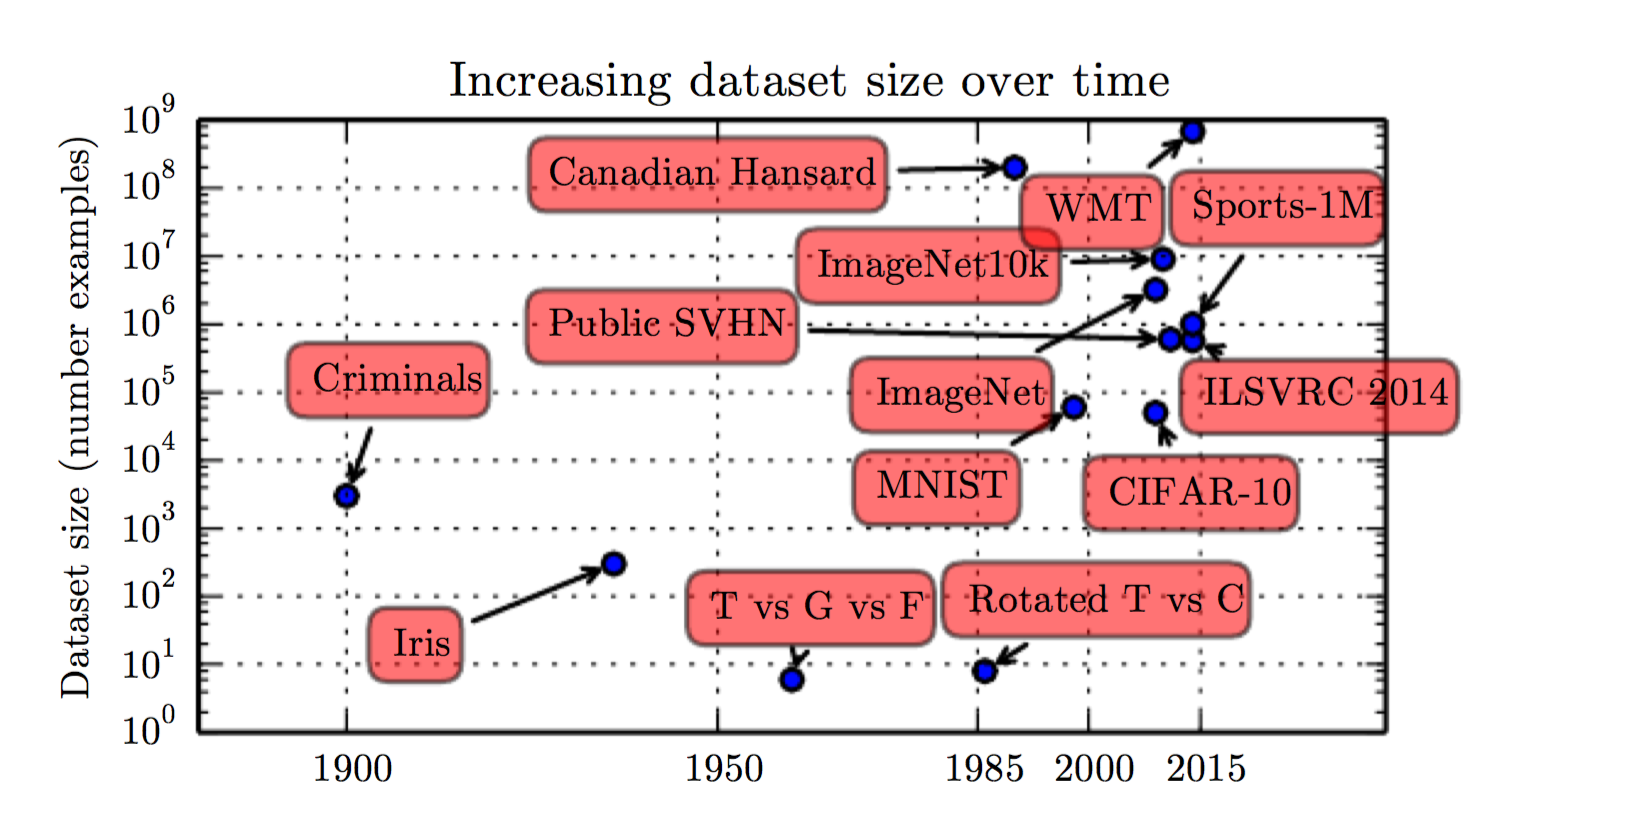
\includegraphics[width=5in]{fig/chap1/1.8.png} 
   \caption{数据集随着时间剧增。在二十世纪初期,统计学家使用成百上千次的手工编译研究数据集。在二十世纪五十年代到八十年代期间,受生物学启发的机器学习先驱经常使用的是小的、合成的数据集,比如信件的低分辨率位图,这些数据的使用是为了减少计算量的基础上使用神经网络实现特定功能。在二十世纪八十年代到九十年代,机器学习变得更加偏统计,并且开始使用万量级的数据集,比如MNIST(如\ref{fig:1.9})就是手写数字的扫描。在二十一世纪的前十年,出现了更多更复杂的数据集也是在这个量级,比如CIFAR-10就在持续的增加。在二十一世纪一零年代的前半部分,从十万到千万量级的更大的数据集完全的改变了深度学习能力的界限。这些数据集包括Street View House Numbers,不同版本的ImageNet,Sports-1M等。在图的顶端我们可以看到翻译句子的数据集,比如由Canadian Hansard构造的IBM数据集,还有WMT2014英法翻译数据集等都远超了其他数据集的量级。}
   \label{fig:1.8}
\end{figure}


\begin{figure}[htbp] %  figure placement: here, top, bottom, or page
   \centering
   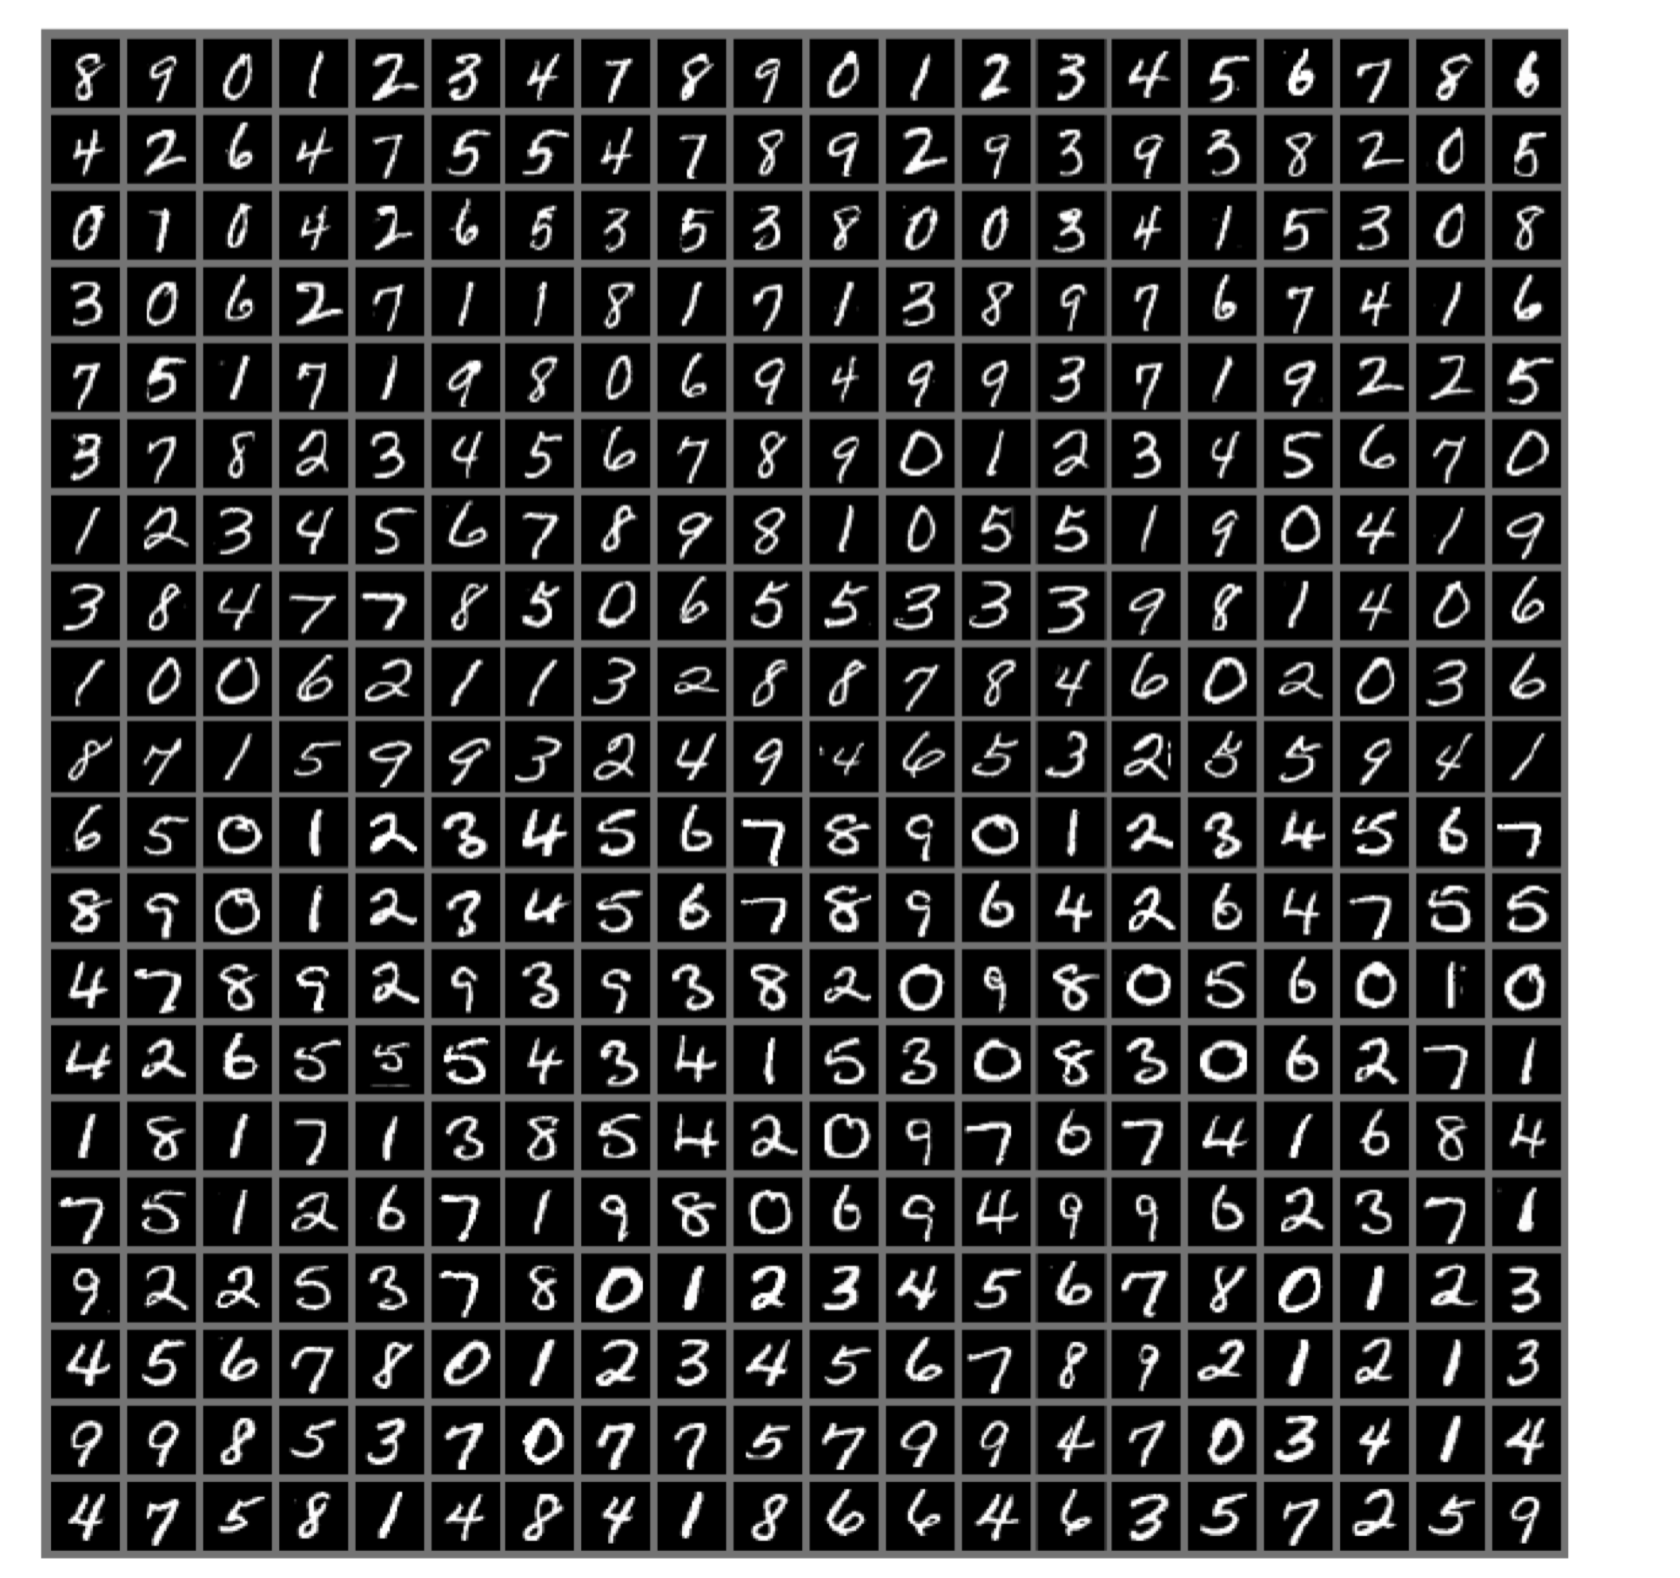
\includegraphics[width=4in]{fig/chap1/1.9.png} 
   \caption{MNIST数据集的示例。“NIST”意思是国家标准技术研究所,就是一开始收集这些数据的机构。“M”意思是“改变的”,因为这批数据为了使得机器学习算法更简单的应用进行了预处理。MNIST数据集中有0-9的手写数字的扫描数据以及相应的标签。这个简单的分类是深度学习研究中最简单也最为广泛使用的测试。尽管这个任务对现代的技术来说很简单,但仍然很流行。Geoffrey Hinton称其为“机器学习的果蝇”,意味着机器学习研究者可以在可控的实验条件下研究他们的算法,正如生物学家经常使用果蝇来帮助研究一样。}
   \label{fig:1.9}
 \end{figure}
   

\subsection{不断变大的模型}
\label{sec:1.2.3}
另一个神经网络现在获得广泛成功的原因是如今我们有计算资源可以计算更大的模型。联结学的主要认知之一就是当有许多的神经元联结在一起的时候动物才能变得智能。一个独立的神经元或者一小组神经元并不是特别有用。


生物的神经元并不总是密集的联结的。如图\ref{fig:1.10},我们的机器学习模型中每个神经元都有一定的连接数,这个数量随着时间变化已经逼近了哺乳动物大脑的连接数的量级。


就神经元的总数而言,神经网络在今天之前的量级小的令人惊讶。

